\chapter{Desenvolvimento do projeto}
\label{chap:metod}
Nesta seção será descrito o procedimento utilizado para construção inicial do portfólio, incluindo as fases conceitual e design.  Será apresentado a ideação do projeto, especificações e as funcionalidades.

\subsection{Metodologia do projeto}
A metodologia adotada para o desenvolvimento do portfólio do cliente seguiu um processo estruturado em etapas, com foco na personalização, usabilidade e alinhamento com os objetivos profissionais do cliente. As fases principais do projeto foram:

1. Levantamento de Requisitos
Inicialmente, foi realizada uma reunião com o cliente para compreender seus objetivos, público-alvo, preferências visuais e conteúdos a serem incluídos no portfólio. Foram levantadas informações como áreas de atuação, projetos realizados, formação, habilidades e experiências profissionais. Esse levantamento guiou toda a concepção do projeto.

2. Planejamento e Estruturação
Com base nos requisitos, foi definida a estrutura do site (mapa de navegação), os principais blocos de conteúdo (sobre, projetos, habilidades, contato etc.) e os recursos funcionais desejados (como formulário de contato, integração com redes sociais ou repositórios de código). Também foram definidas as tecnologias a serem utilizadas no desenvolvimento.

3. Criação do Design
Foi desenvolvido um layout responsivo e personalizado, baseado nas referências visuais fornecidas pelo cliente e nas boas práticas de design. O protótipo foi validado com o cliente antes do início do desenvolvimento para garantir alinhamento com suas expectativas.

4. Desenvolvimento
O desenvolvimento foi feito utilizando tecnologias web modernas. O código foi estruturado visando desempenho, acessibilidade e facilidade de manutenção. Todo o conteúdo foi inserido de forma dinâmica e otimizada para diferentes dispositivos.

5. Testes e Ajustes
Após a finalização do desenvolvimento, foram realizados testes funcionais, de responsividade e compatibilidade com diferentes navegadores e dispositivos. Ajustes finos foram feitos com base no feedback do cliente.
\section{Ideação}
%escrever oq sera apresentado

\subsection{Arquitetura Geral}
Arquitetura do Projeto
A arquitetura do projeto foi planejada para garantir modularidade, escalabilidade, desempenho e facilidade de manutenção. A estrutura contempla tanto os aspectos técnicos quanto organizacionais do sistema, com foco na entrega de um portfólio moderno, responsivo e funcional.
\begin{itemize}


\item 1. Arquitetura de CamadasO projeto foi dividido em camadas lógicas para organizar melhor as responsabilidades:
\item 2. Camada de Apresentação (Front-end):Responsável pela interface do usuário e experiência de navegação. Desenvolvida com tecnologias web como HTML5, CSS3. Esta camada consome os dados estruturados (projetos, informações pessoais etc.) e os exibe de forma dinâmica.
\item 3. Camada de Dados (Content Layer):Os dados do portfólio ou integrados a um CMS leve para permitir atualizações sem editar código.
\item 4. Camada de Publicação/Servidor (Back-end e Hosting):Em projetos estáticos, esta camada pode ser composta apenas por um serviço de hospedagem como GitHub Pages. 

A arquitetura contempla o uso de design responsivo com media queries e classes utilitárias, garantindo compatibilidade com dispositivos móveis, tablets e desktops. Padrões de acessibilidade como contraste de cores, semântica HTML e navegação por teclado também foram considerados.

\end{itemize}

 	



%desdobramento da função qualidade
% \subsection{Quality Function Deployment}
% \textit{Quality Function Deployment} é uma ferramenta de qualidade que auxilia na conversão das demandas do cliente em características de qualidade do produto. Dessa forma, no primeiro ciclo do QFD foram analisados os requisistos do cliente e os requisitos técnicos necessários, sinalizando os pontos mais importantes e as relações entre estes. O resultado foi exposto na \ref{fig:QFD}

% \begin{figure} [h!]	
%     \centering
%     \caption{ Primeiro ciclo QFD}
%     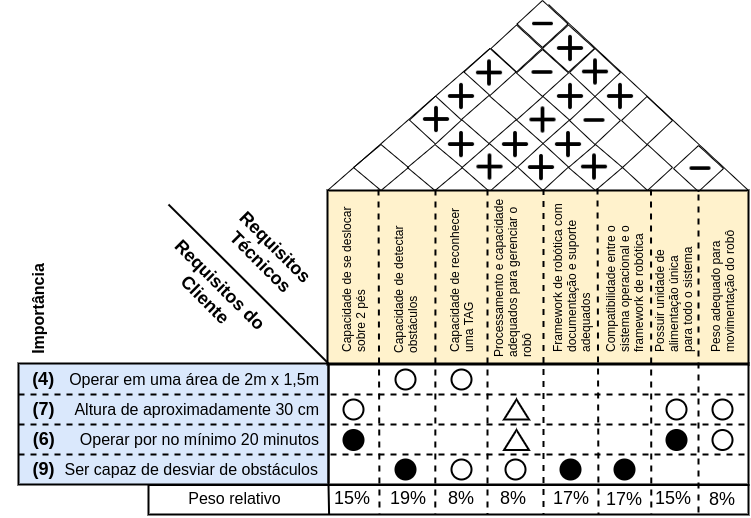
\includegraphics[width=0.8\textwidth]{Figures/QFD}
%     \caption*{Fonte: Autoria própria.}
%     \label{fig:QFD}
% \end{figure}
%  Através do QFD foi possível observar 

% % %--------- NEW SECTION ----------------------
% % \section{Interface do Usuário}
% % \label{sec:ui}
% % \lipsum[1]

% % %--------- NEW SECTION ----------------------
% % \section{Simulação do sistema}
% % \label{sec:sim}
% % \lipsum[2-4]
\subsection{Modelagem dos processos}

\begin{figure} [h!]	
    \centering

    \caption{Modelo esquemático dos processos}
    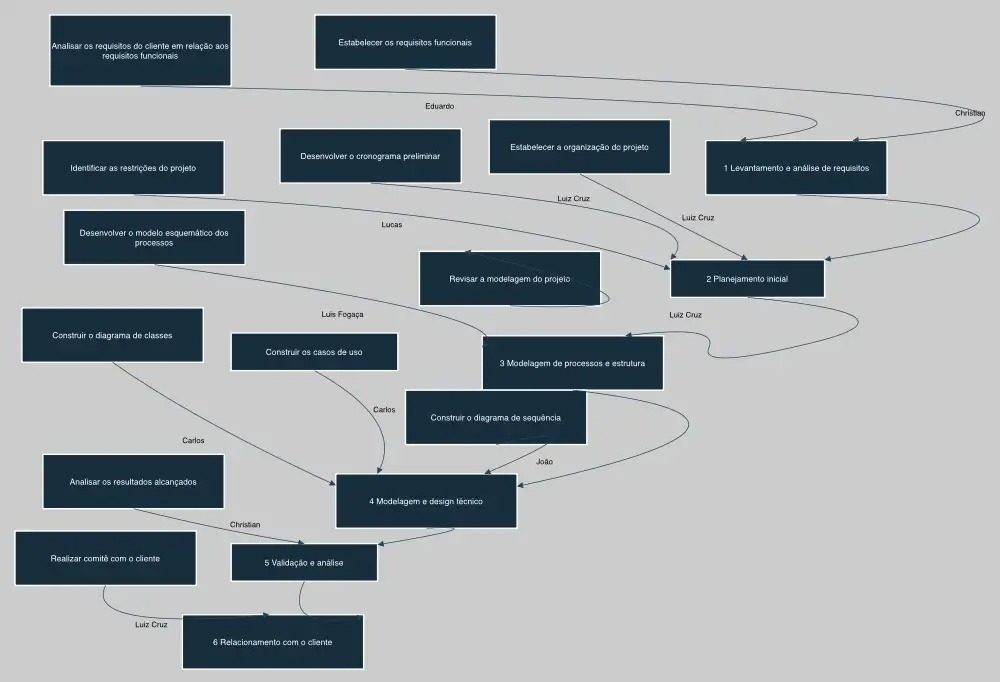
\includegraphics[width=0.9\textwidth]{Figures/Modelagem-dos-processos.jpg}
    \caption*{Fonte: Autoria própria.}
    \label{fig:Modelagem-dos-processos}
\end{figure}